\chapter{ExtendedShortcut}\label{chap:appendixC}

This appendix provides grid search results to determine the optimal hyperparameters for the \myglsentry{saextendedshct} algorithm.

\begin{figure} [htp]
    \centering
    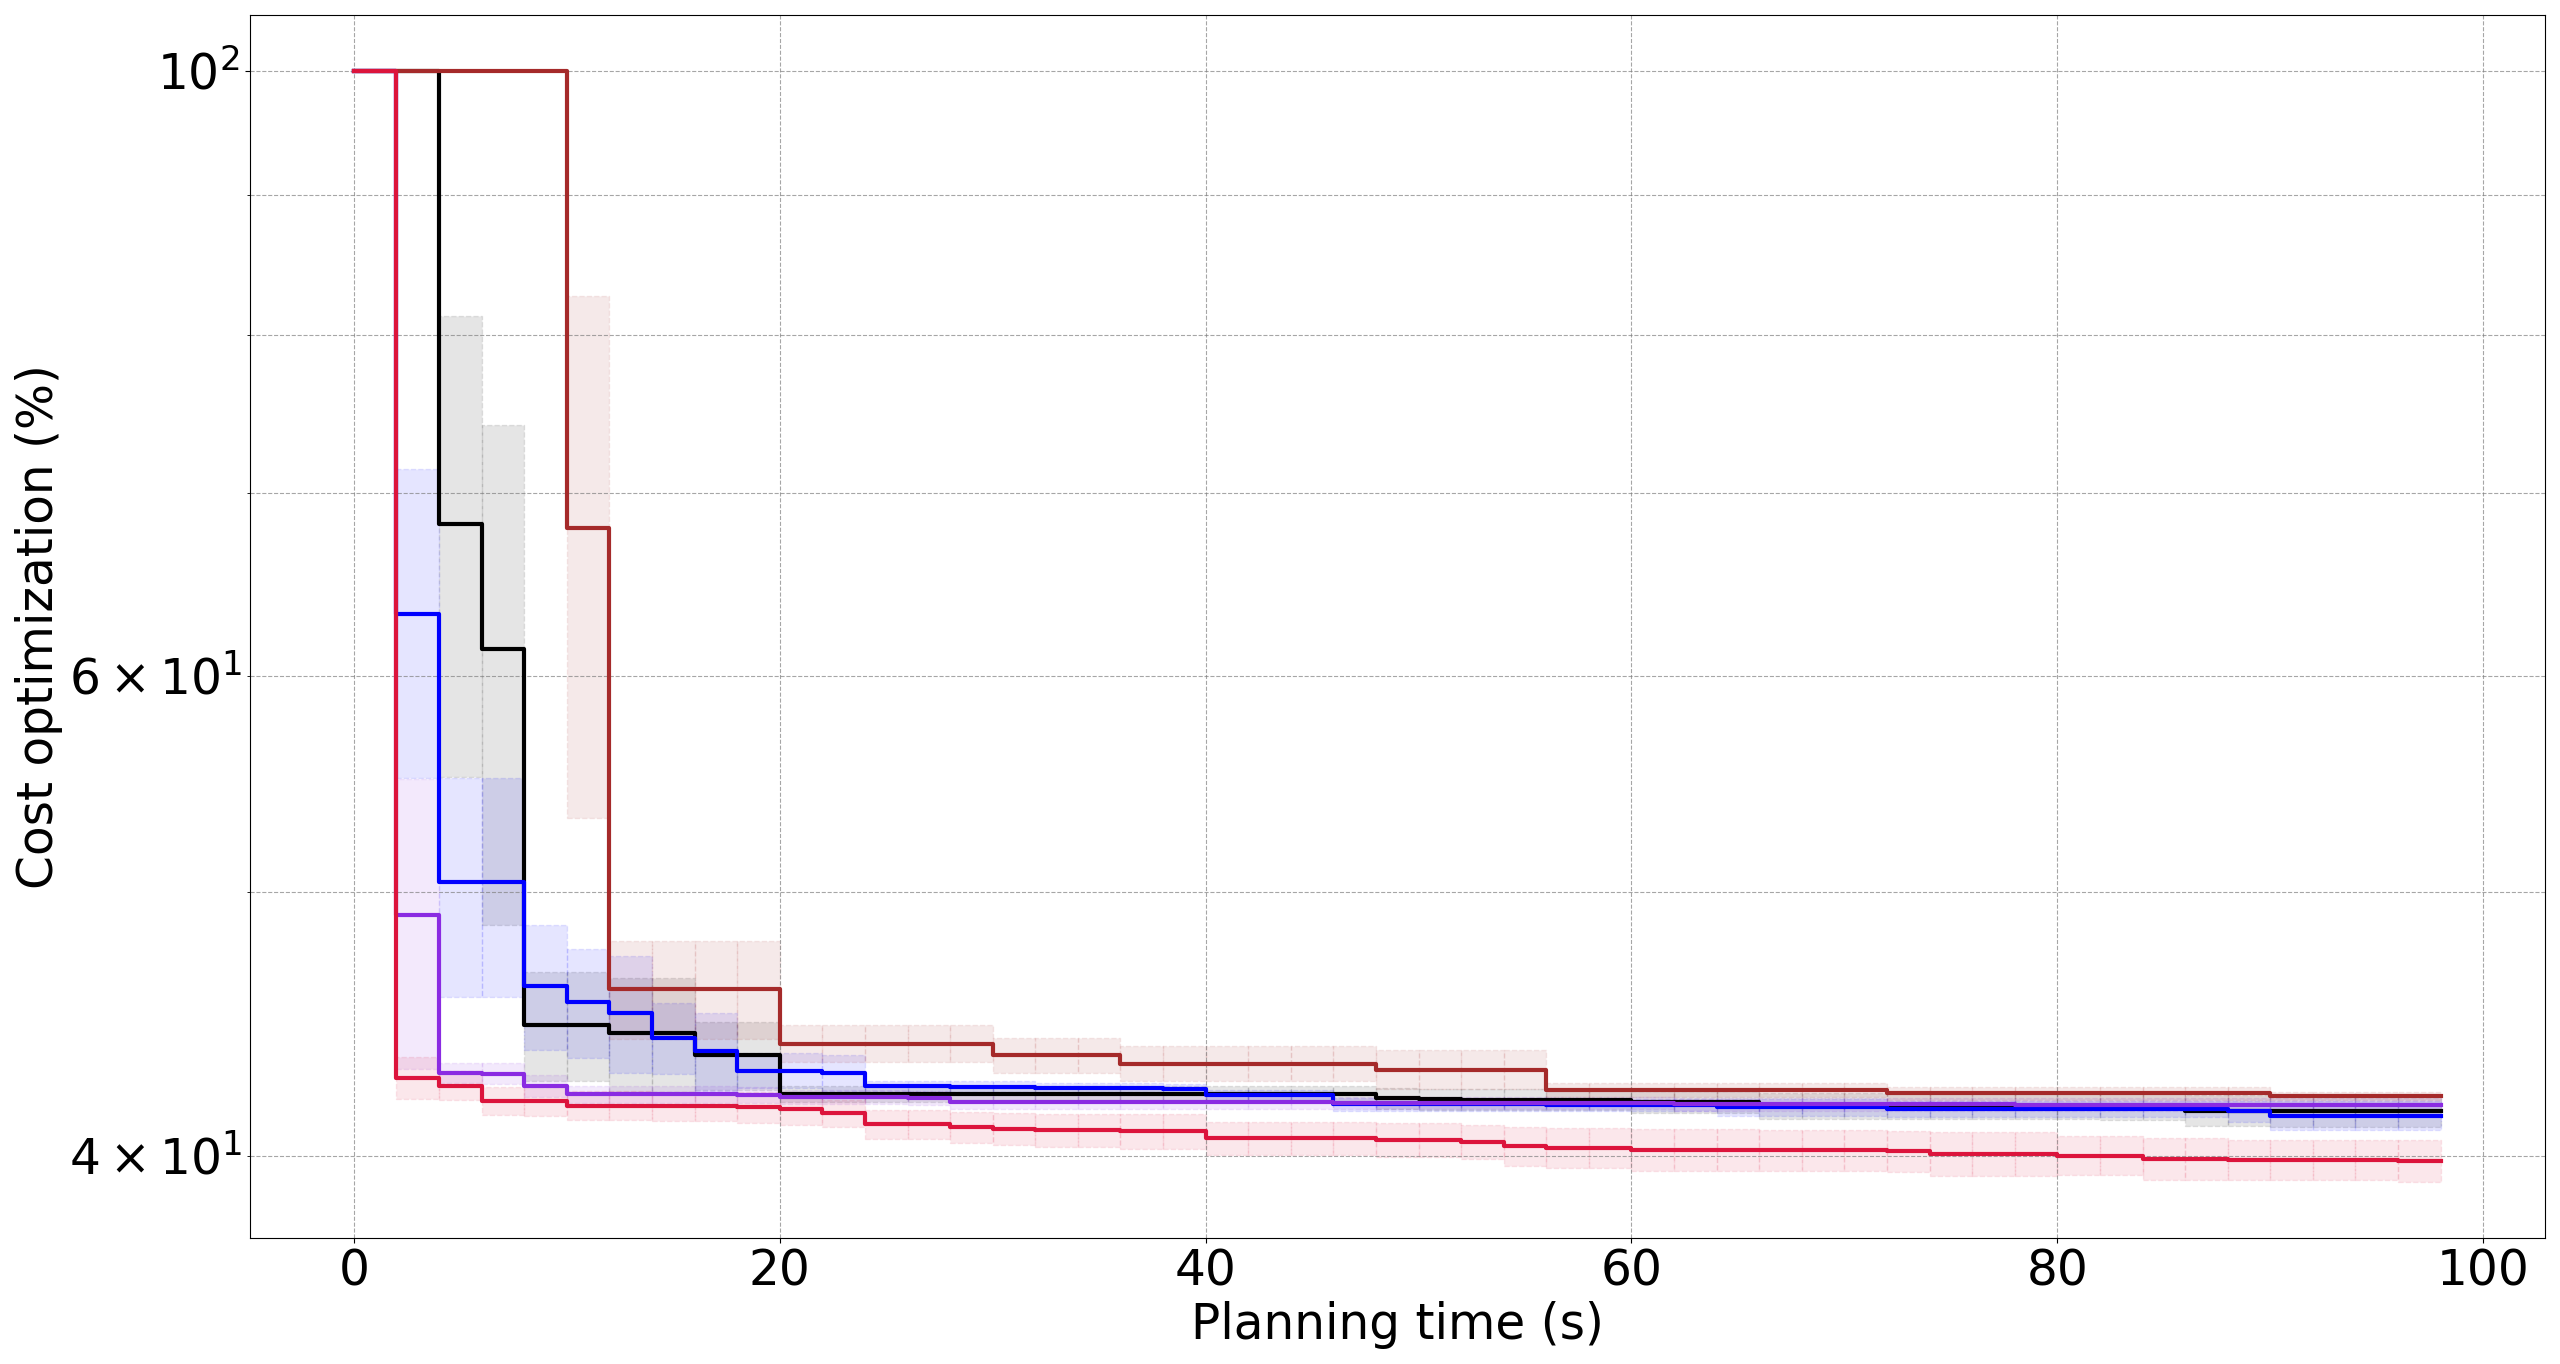
\includegraphics[width=0.9\linewidth]{figures/appendix/uniform_radius_0_01.png} \\
    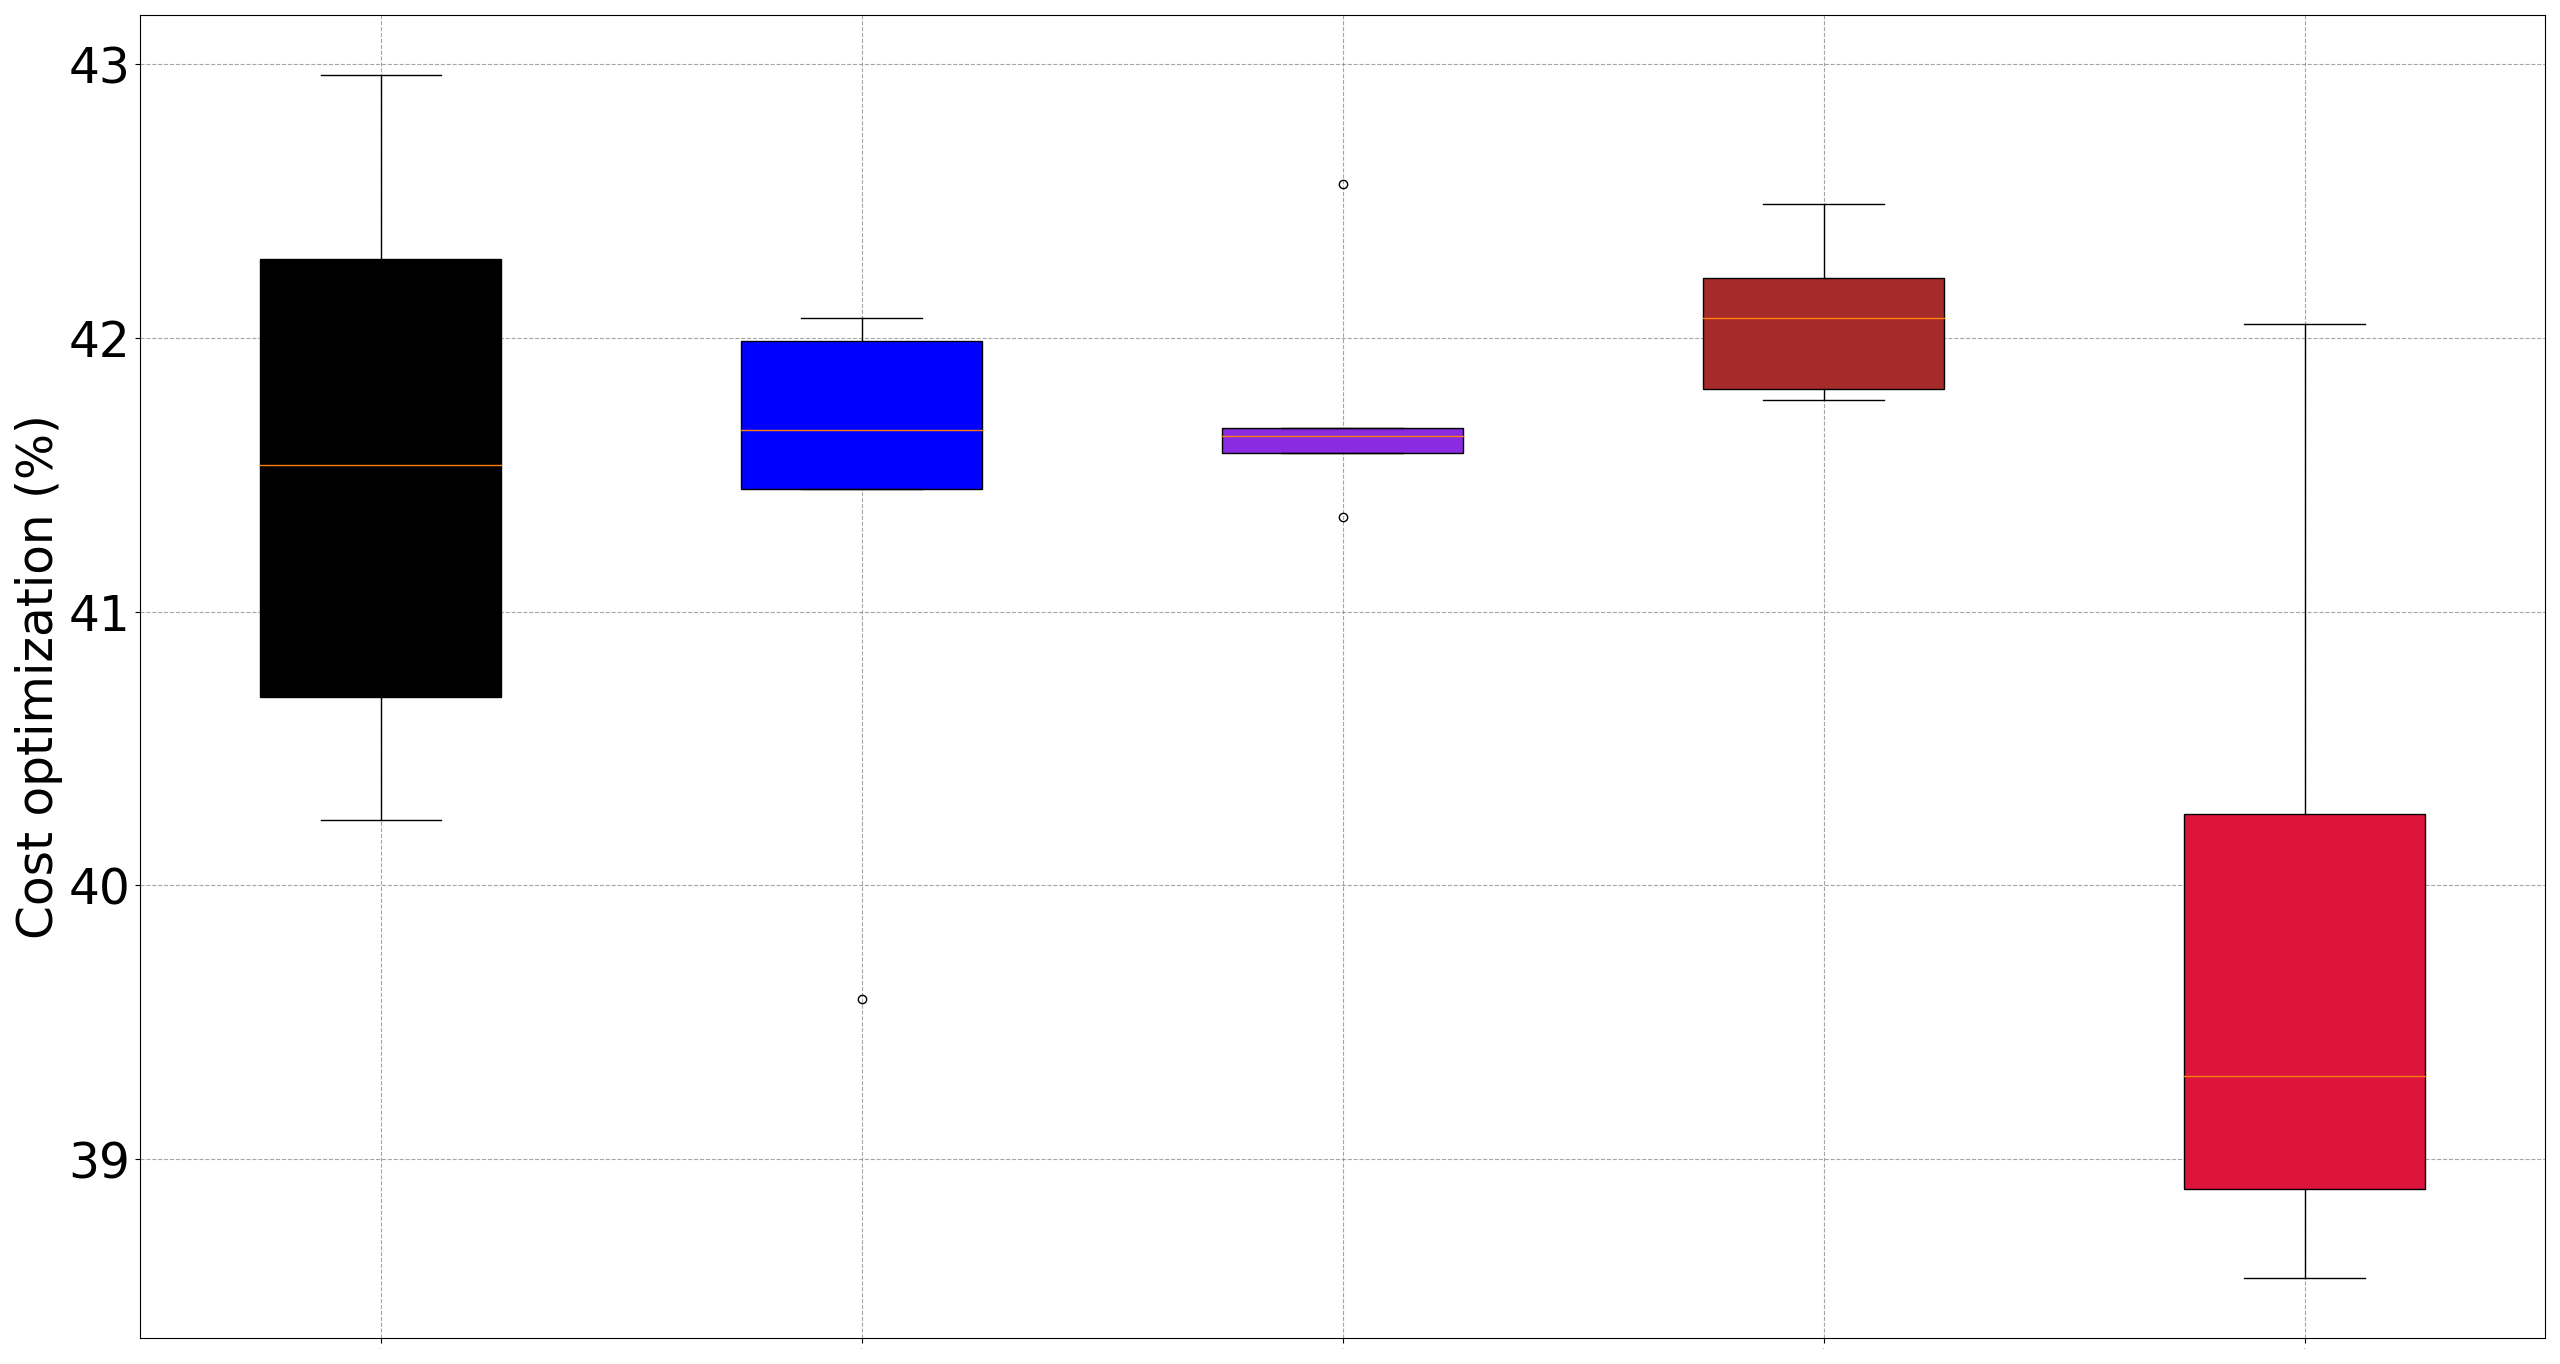
\includegraphics[width=0.9\linewidth]{figures/appendix/bplot_uniform_radius_0_01.png}
    \caption{Cost optimization results using a uniform sampling and a radius $\delta = 0.01$, averaged over 10 plans in a free space environment. 
    The standard deviation is represented as an envelope around the mean curves.
    The red curve corresponds to $K = 1$, the purple curve to $K = 2$, the blue one to $K = 3$, the black to $K = 5$, and the brown curve to $K = 10$.}%
    \label{fig:uniform_radius_0_01}%
\end{figure}

\begin{figure} [htp]
    \centering
    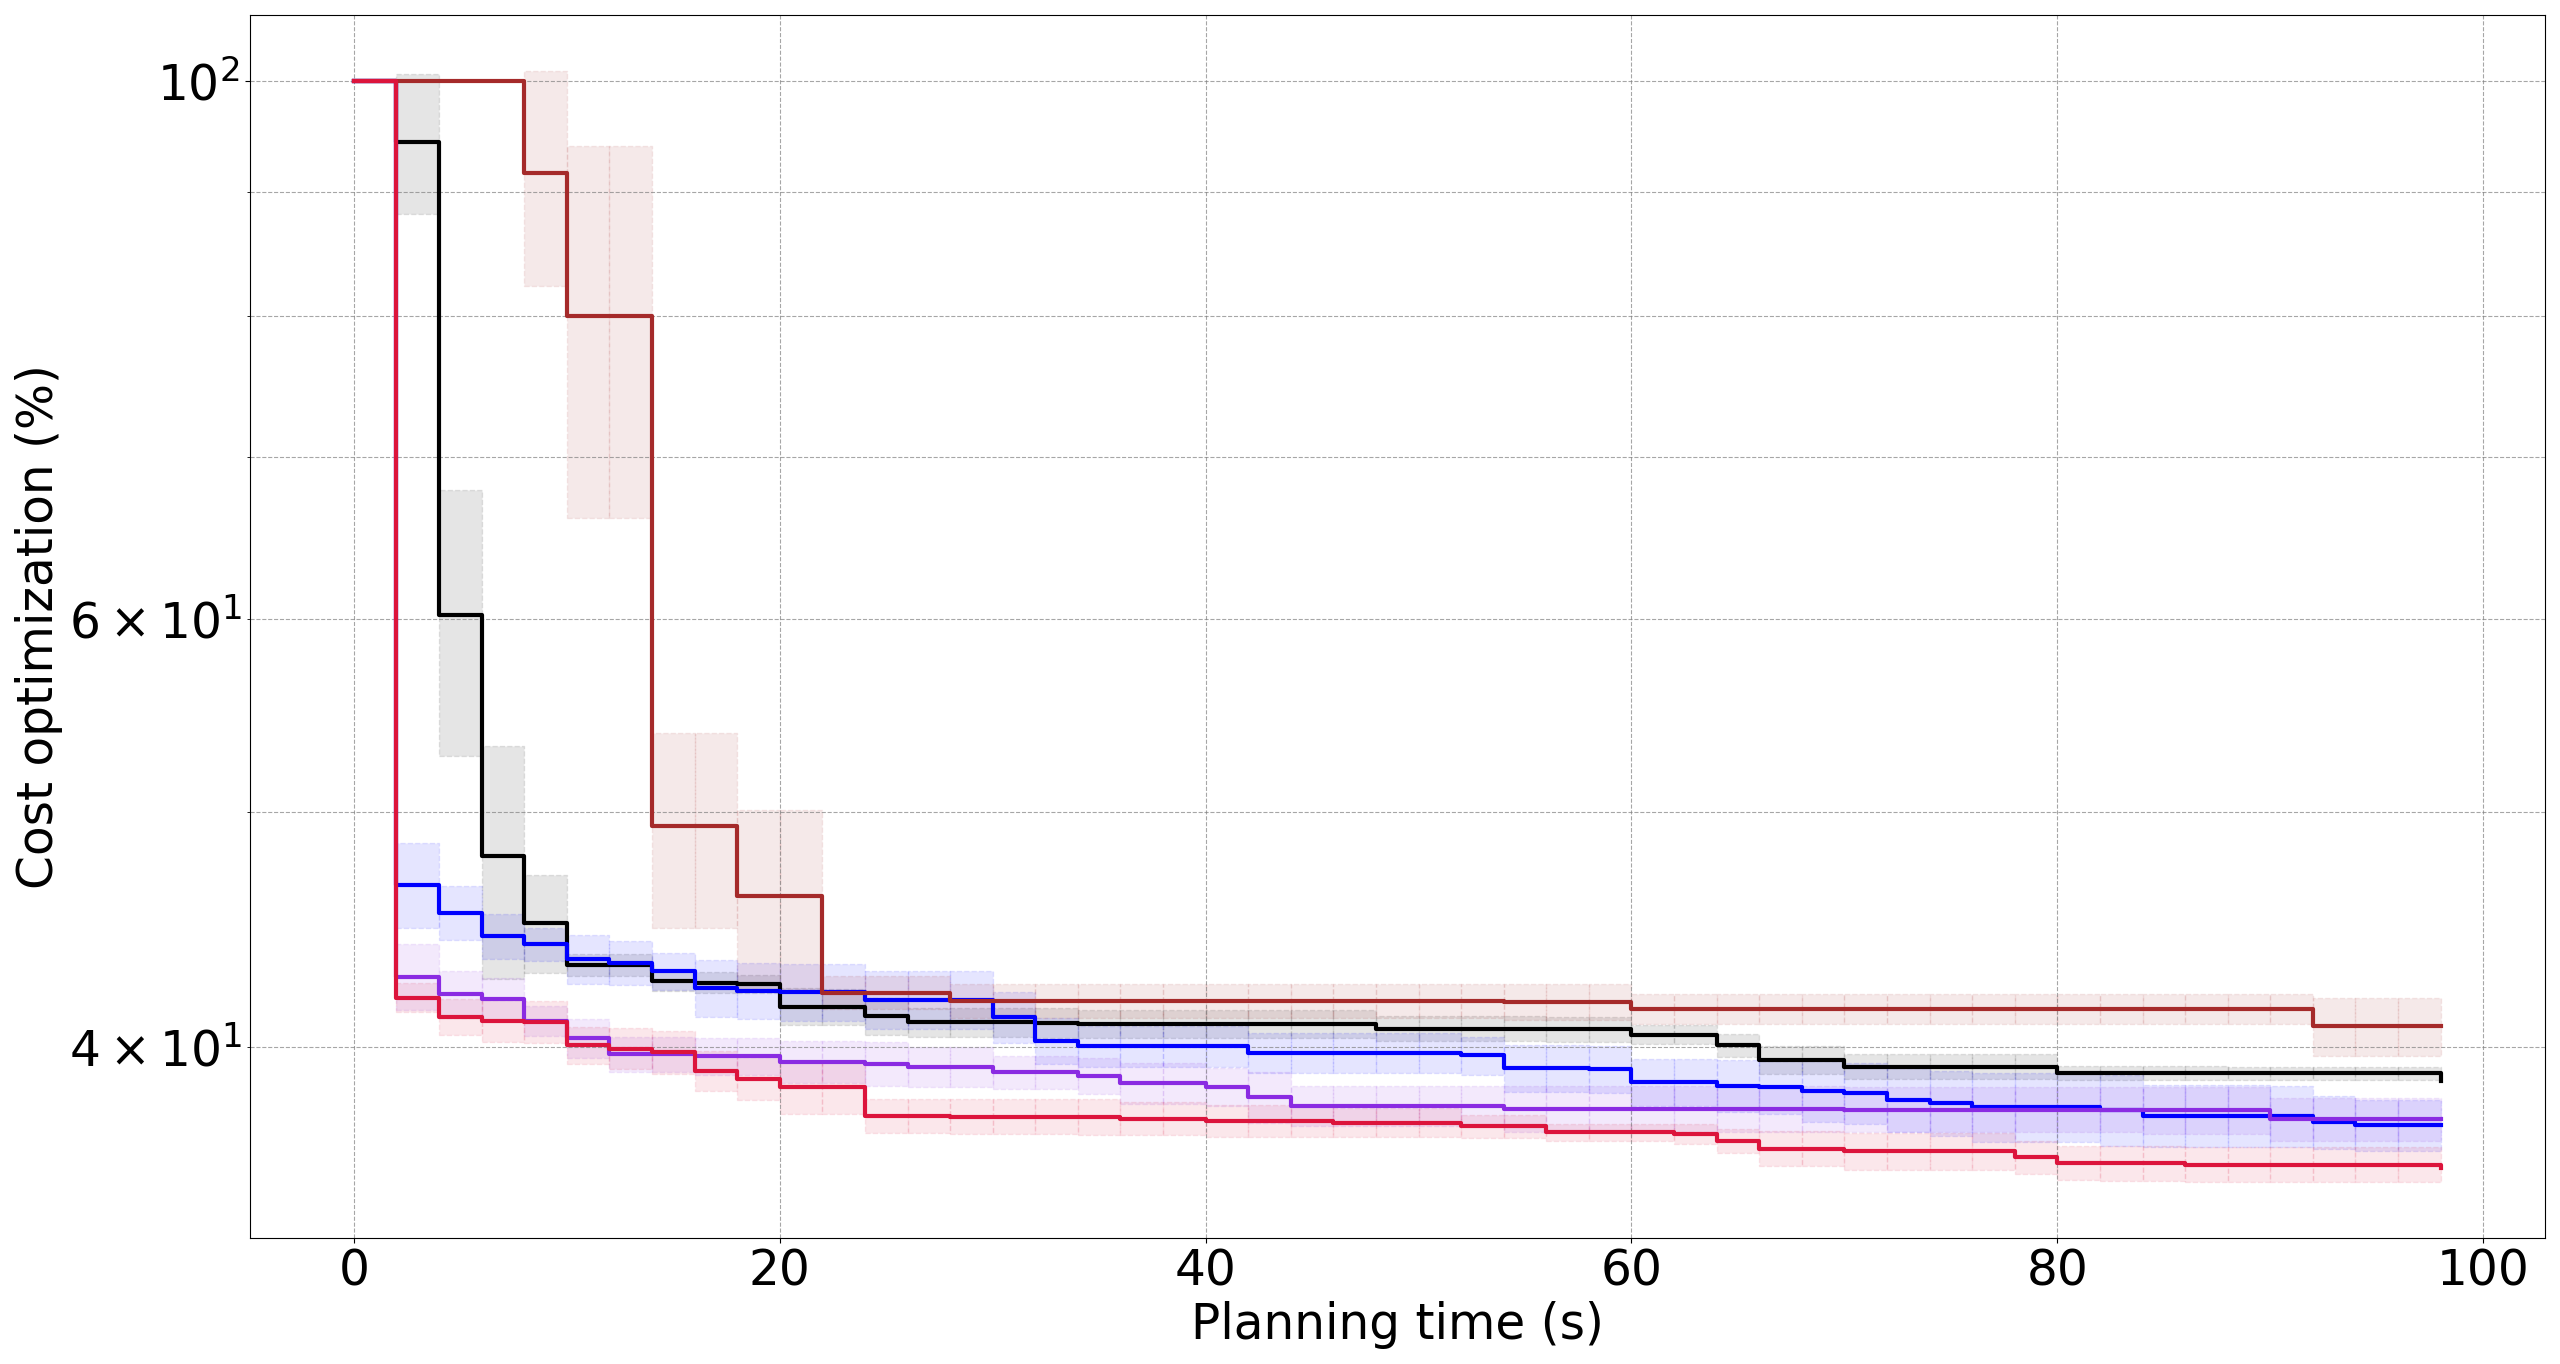
\includegraphics[width=0.9\linewidth]{figures/appendix/uniform_radius_0_1.png} \\
    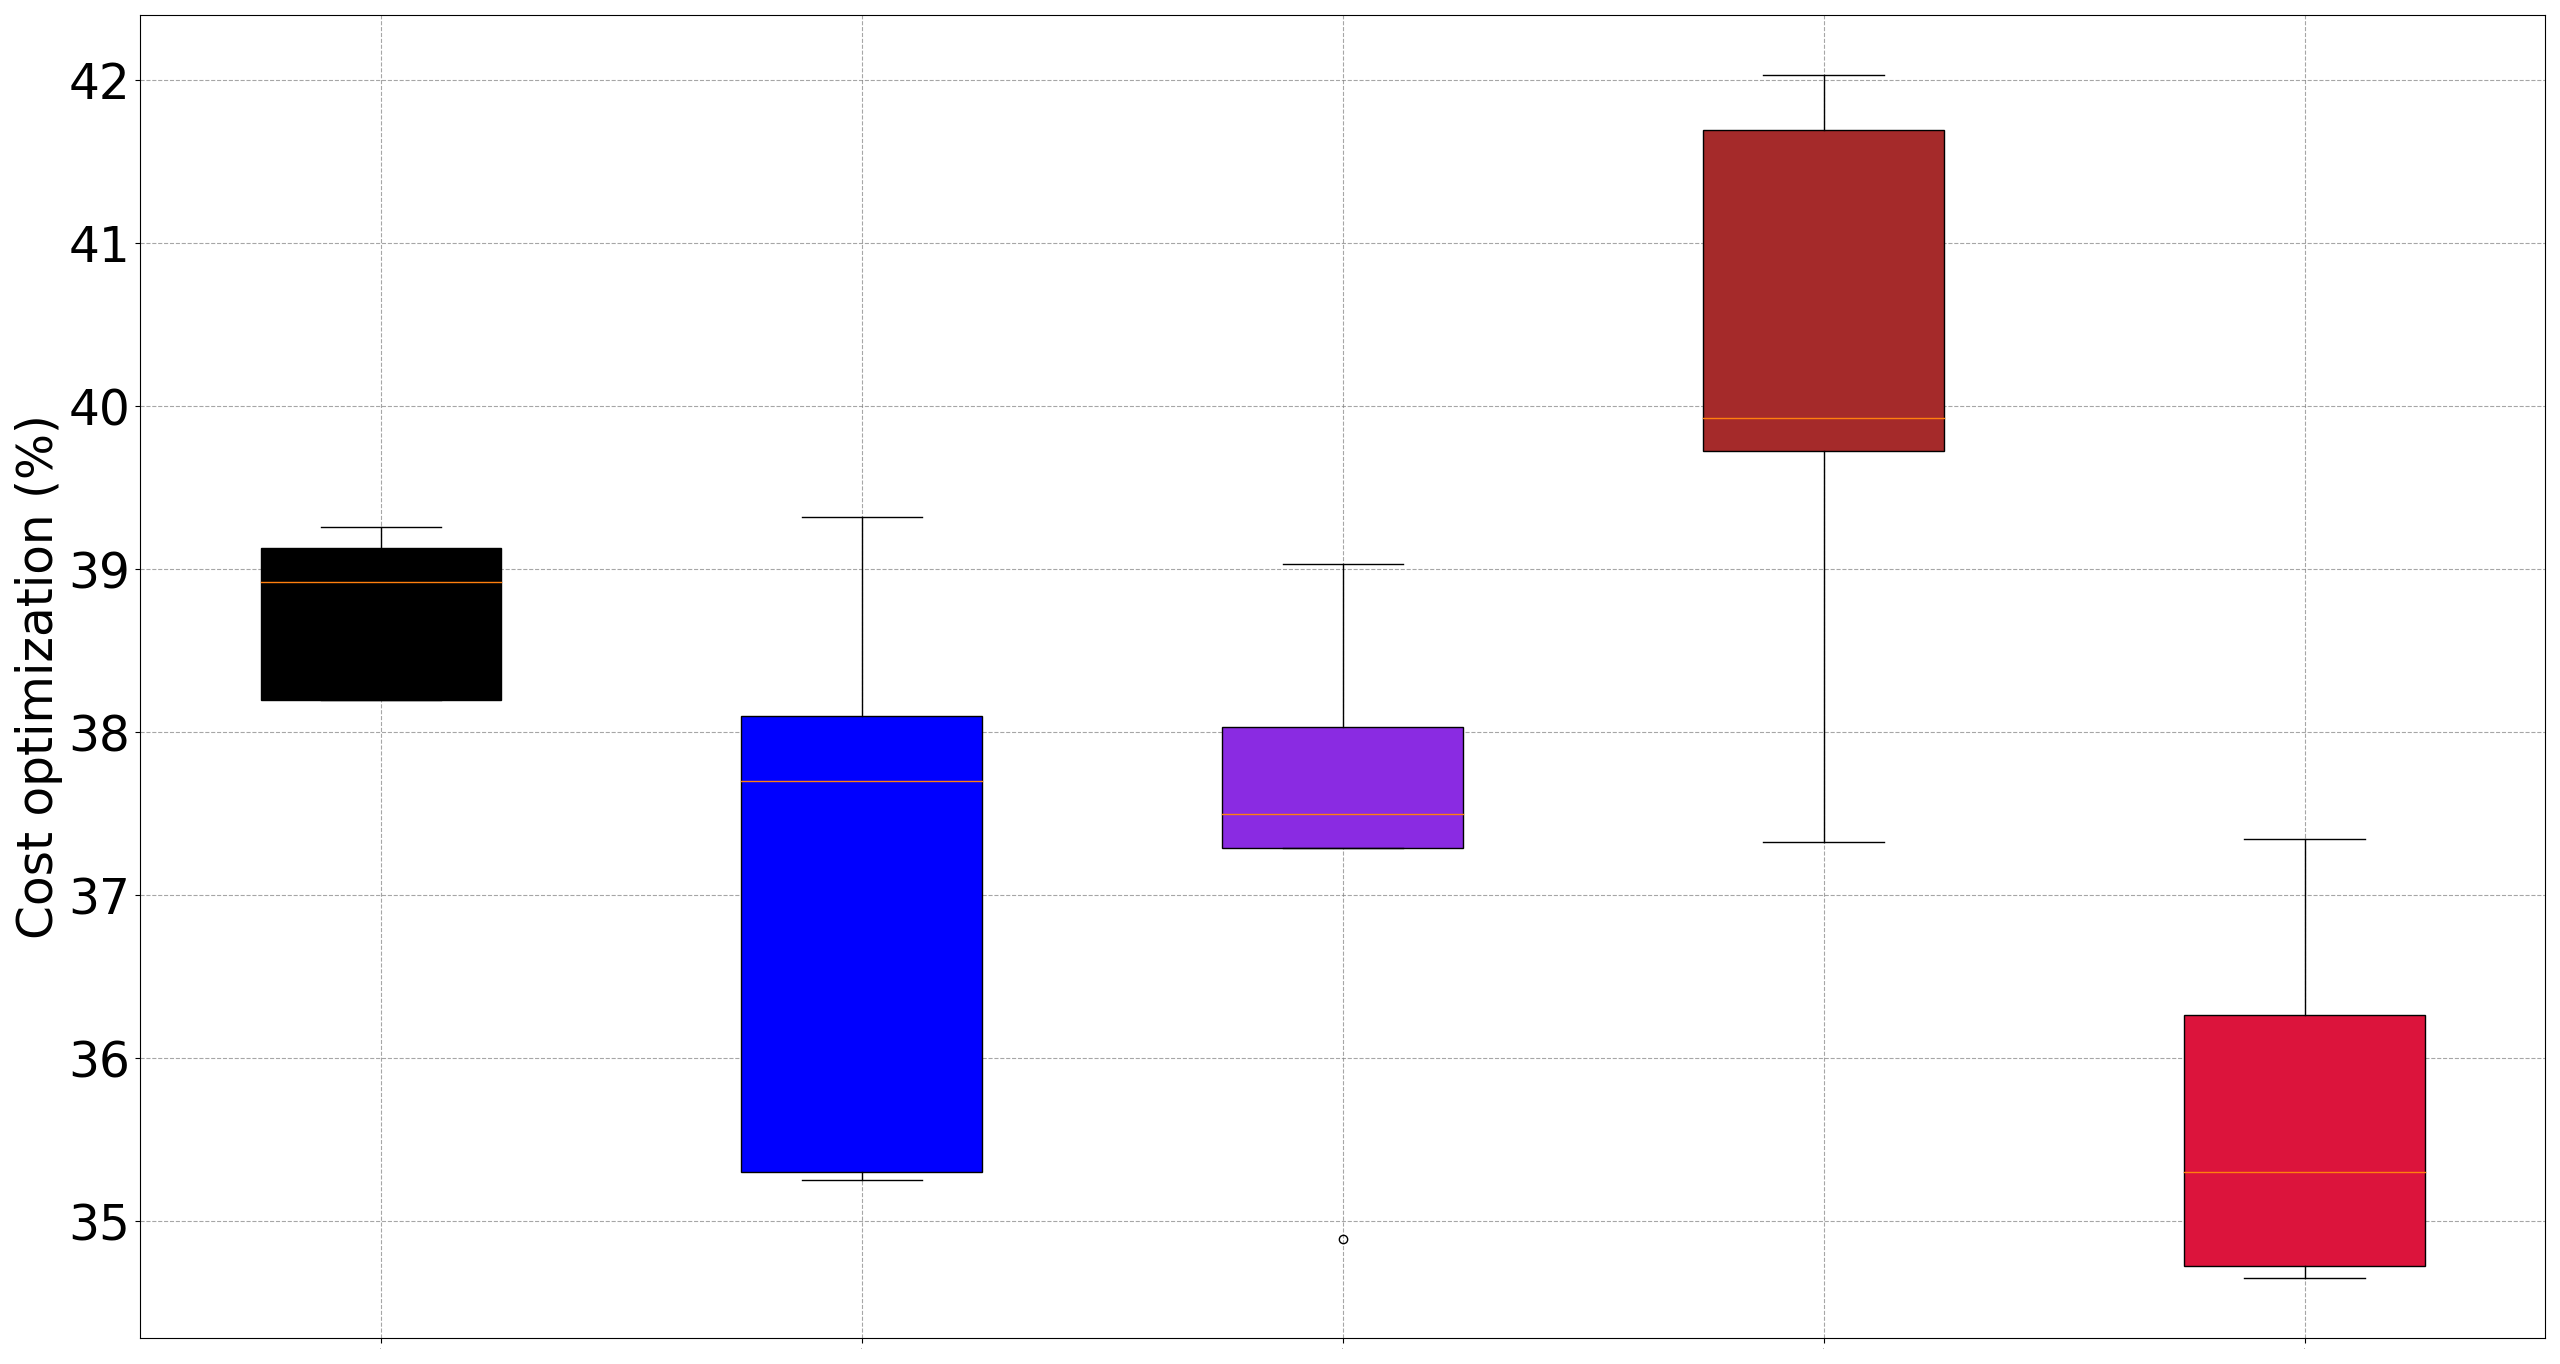
\includegraphics[width=0.9\linewidth]{figures/appendix/bplot_uniform_radius_0_1.png}
    \caption{Cost optimization results using a uniform sampling and a radius $\delta = 0.1$, averaged over 10 plans in a free space environment. 
    The standard deviation is represented as an envelope around the mean curves.
    The red curve corresponds to $K = 1$, the purple curve to $K = 2$, the blue one to $K = 3$, the black to $K = 5$, and the brown curve to $K = 10$.}%
    \label{fig:uniform_radius_0_1}%
\end{figure}

\begin{figure} [htp]
    \centering
    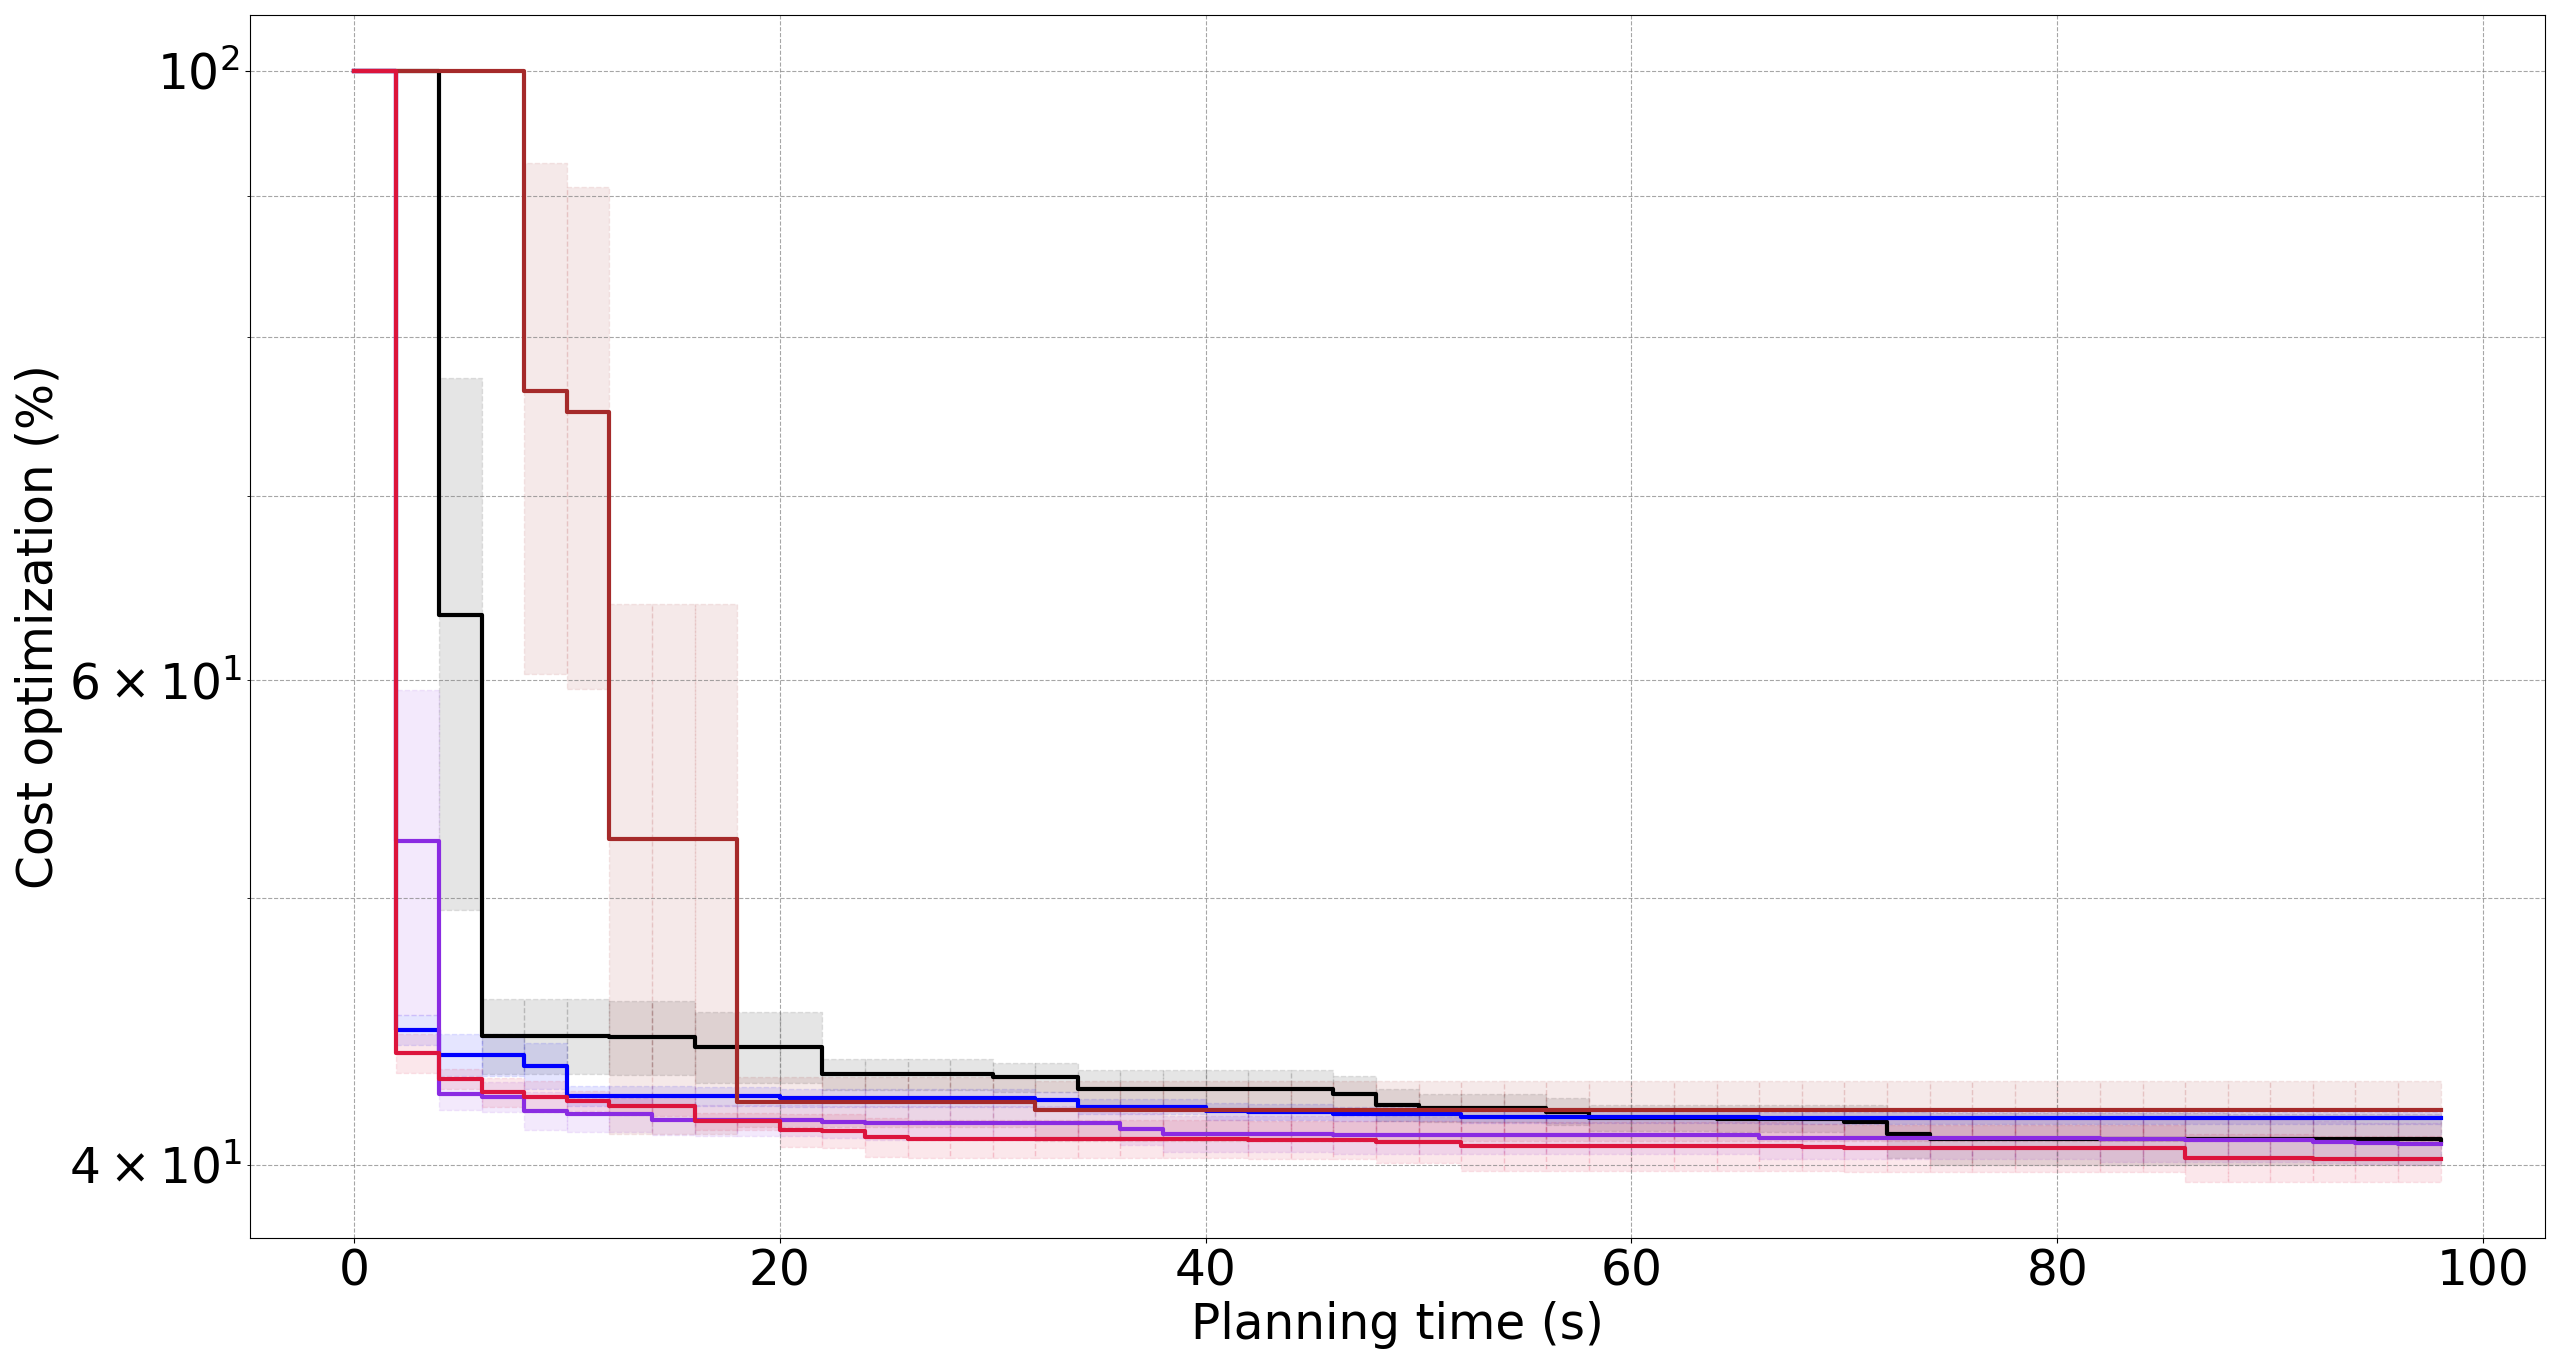
\includegraphics[width=0.9\linewidth]{figures/appendix/gaussian_radius_0_01.png} \\
    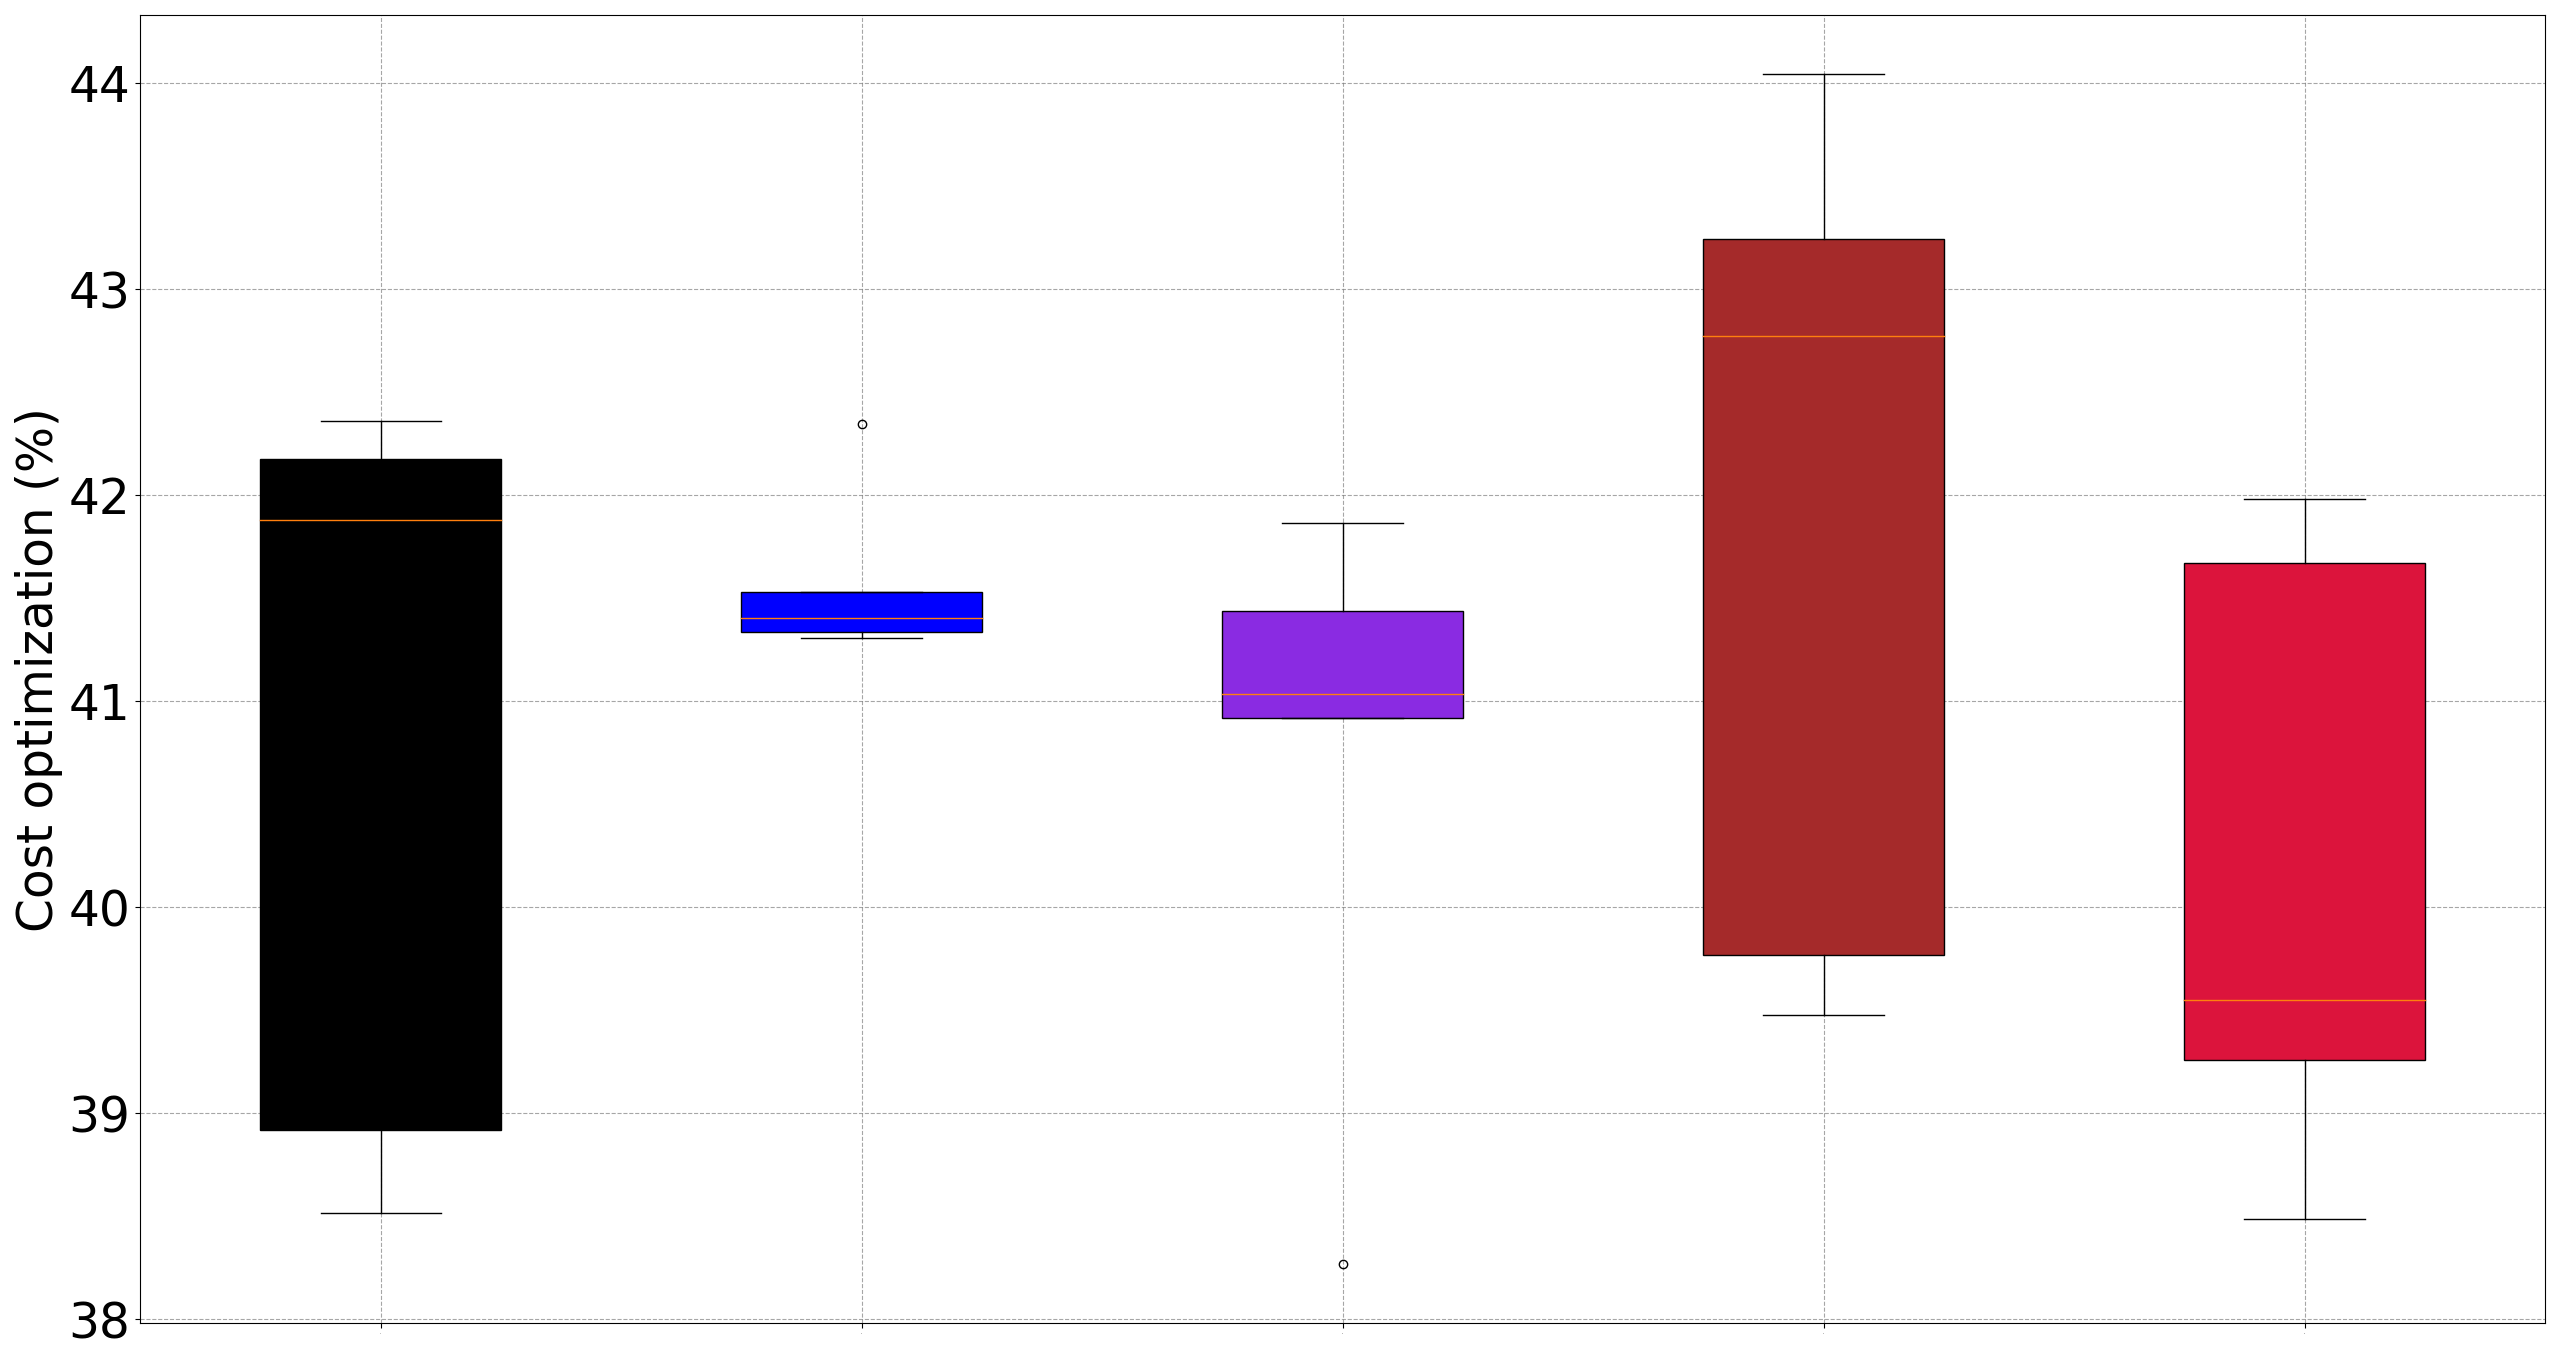
\includegraphics[width=0.9\linewidth]{figures/appendix/bplot_gaussian_radius_0_01.png}
    \caption{Cost optimization results using a Gaussian sampling with a standard deviation $\delta = 0.01$, averaged over 10 plans in a free space environment. 
    The standard deviation is represented as an envelope around the mean curves.
    The red curve corresponds to $K = 1$, the purple curve to $K = 2$, the blue one to $K = 3$, the black to $K = 5$, and the brown curve to $K = 10$.}%
    \label{fig:gaussian_radius_0_01}%
\end{figure}

\begin{figure} [htp]
    \centering
    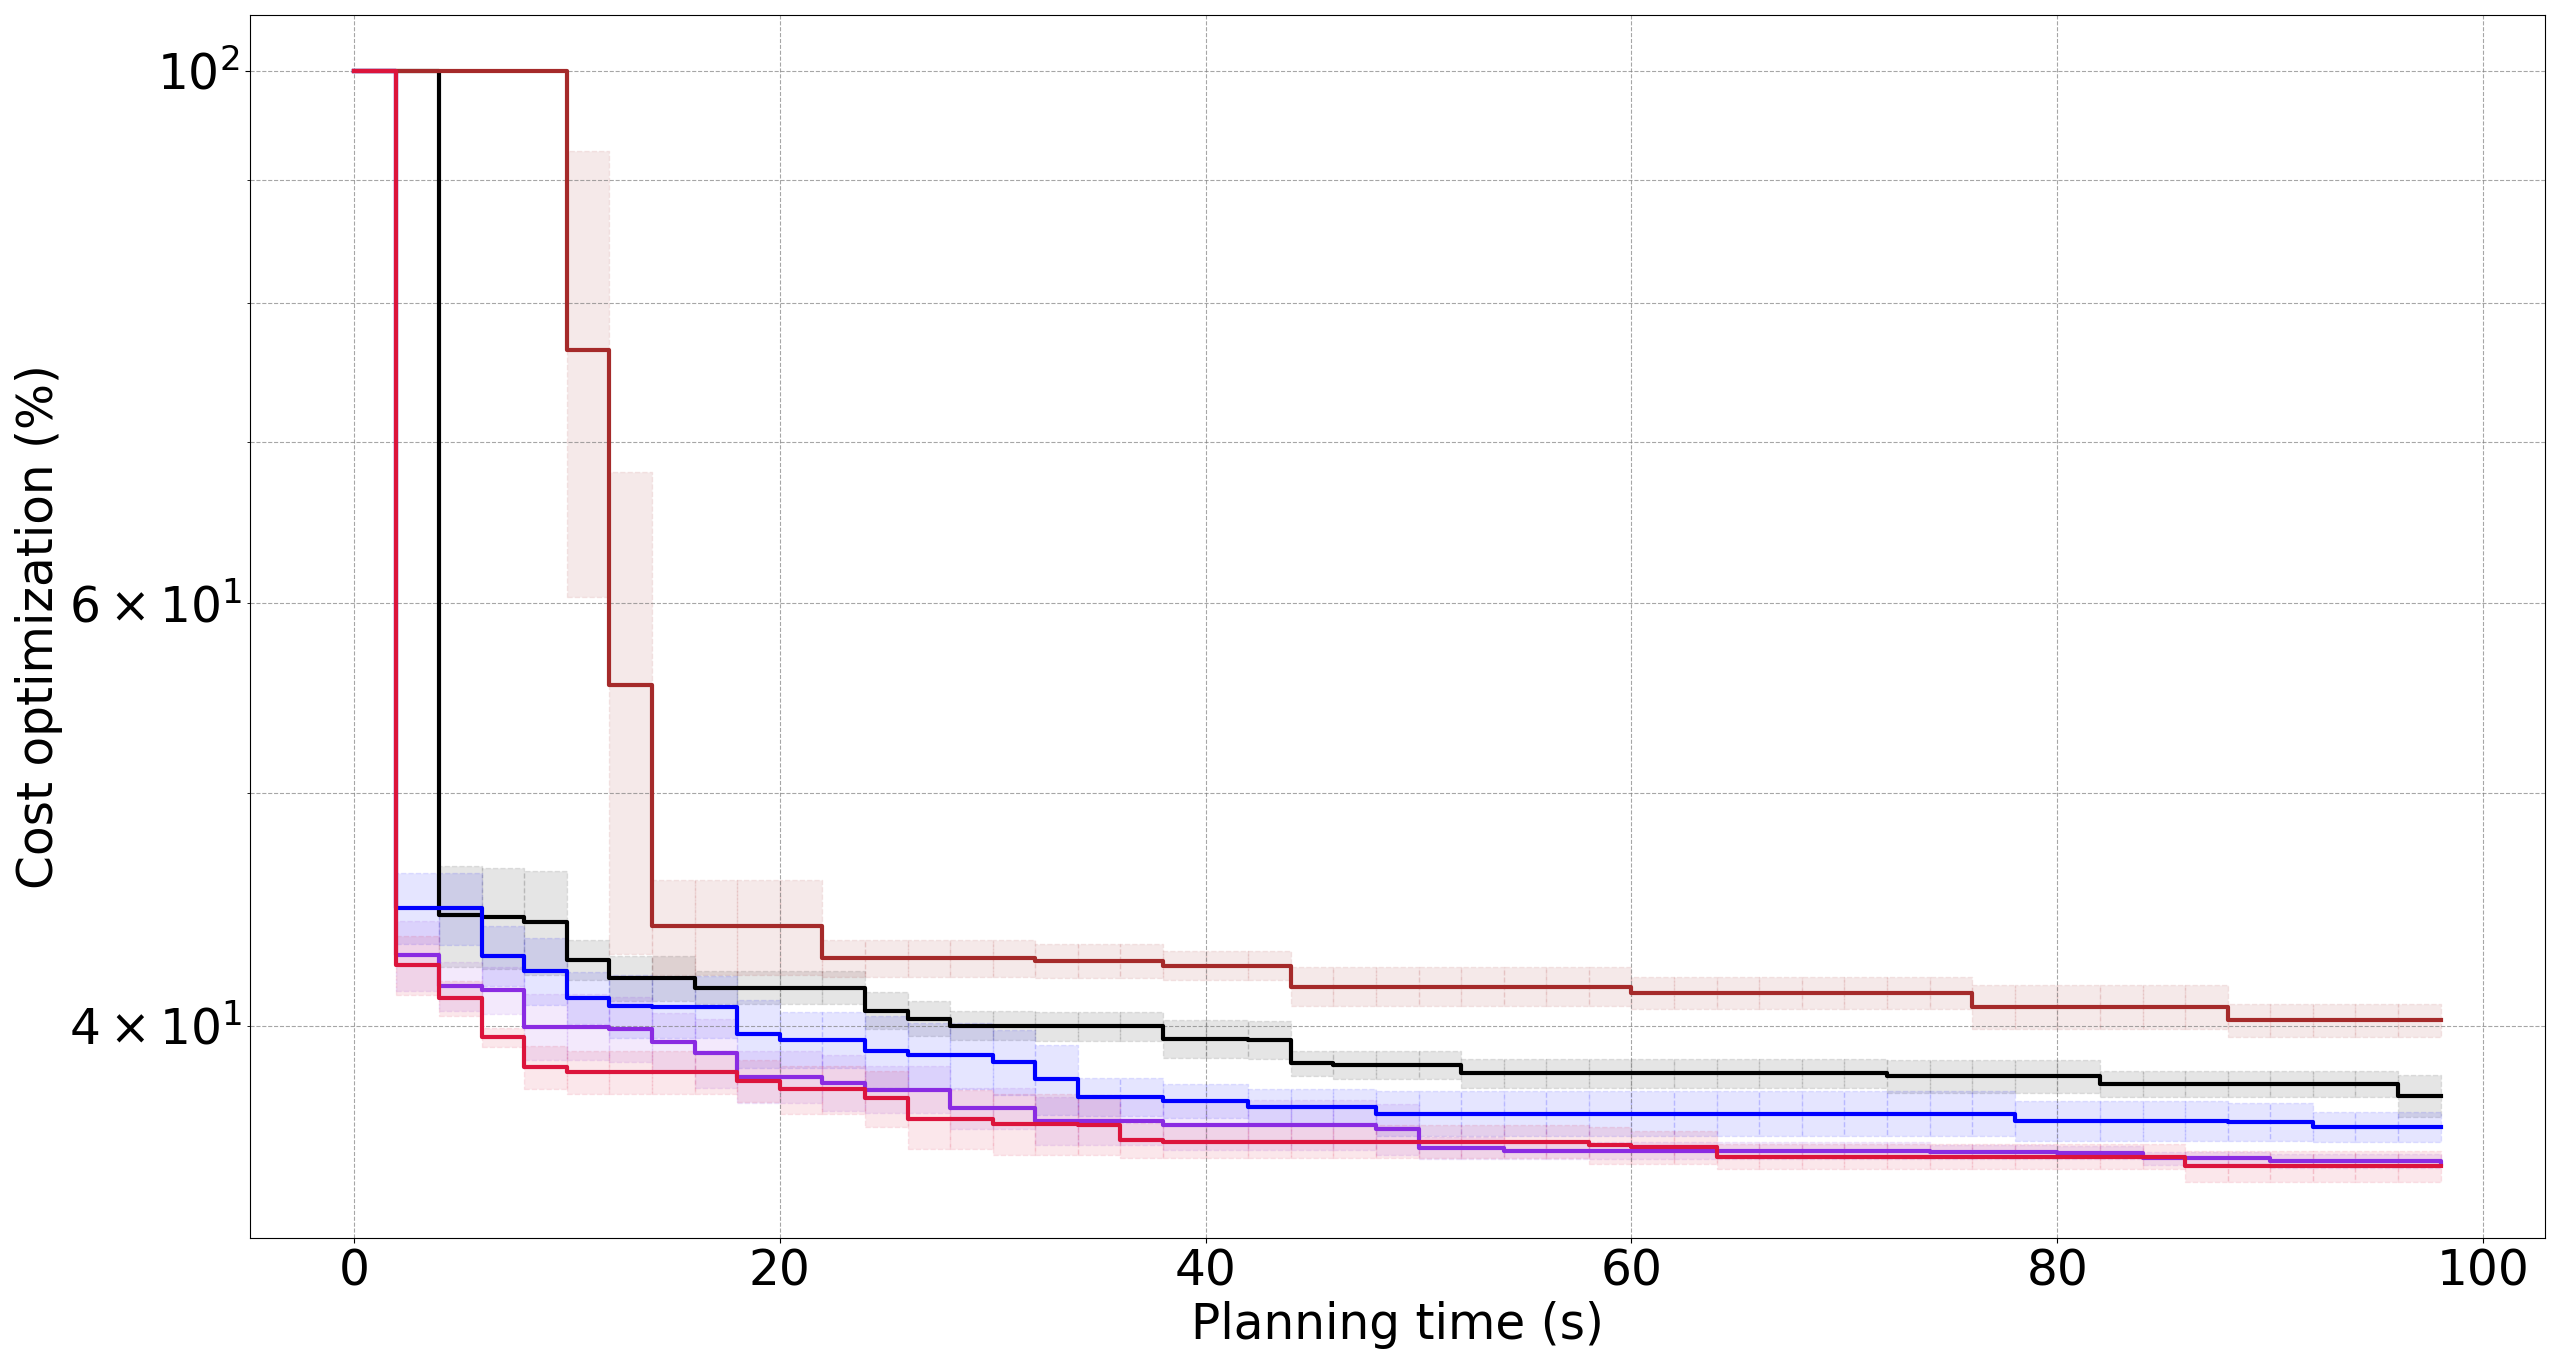
\includegraphics[width=0.9\linewidth]{figures/appendix/gaussian_radius_0_1.png} \\
    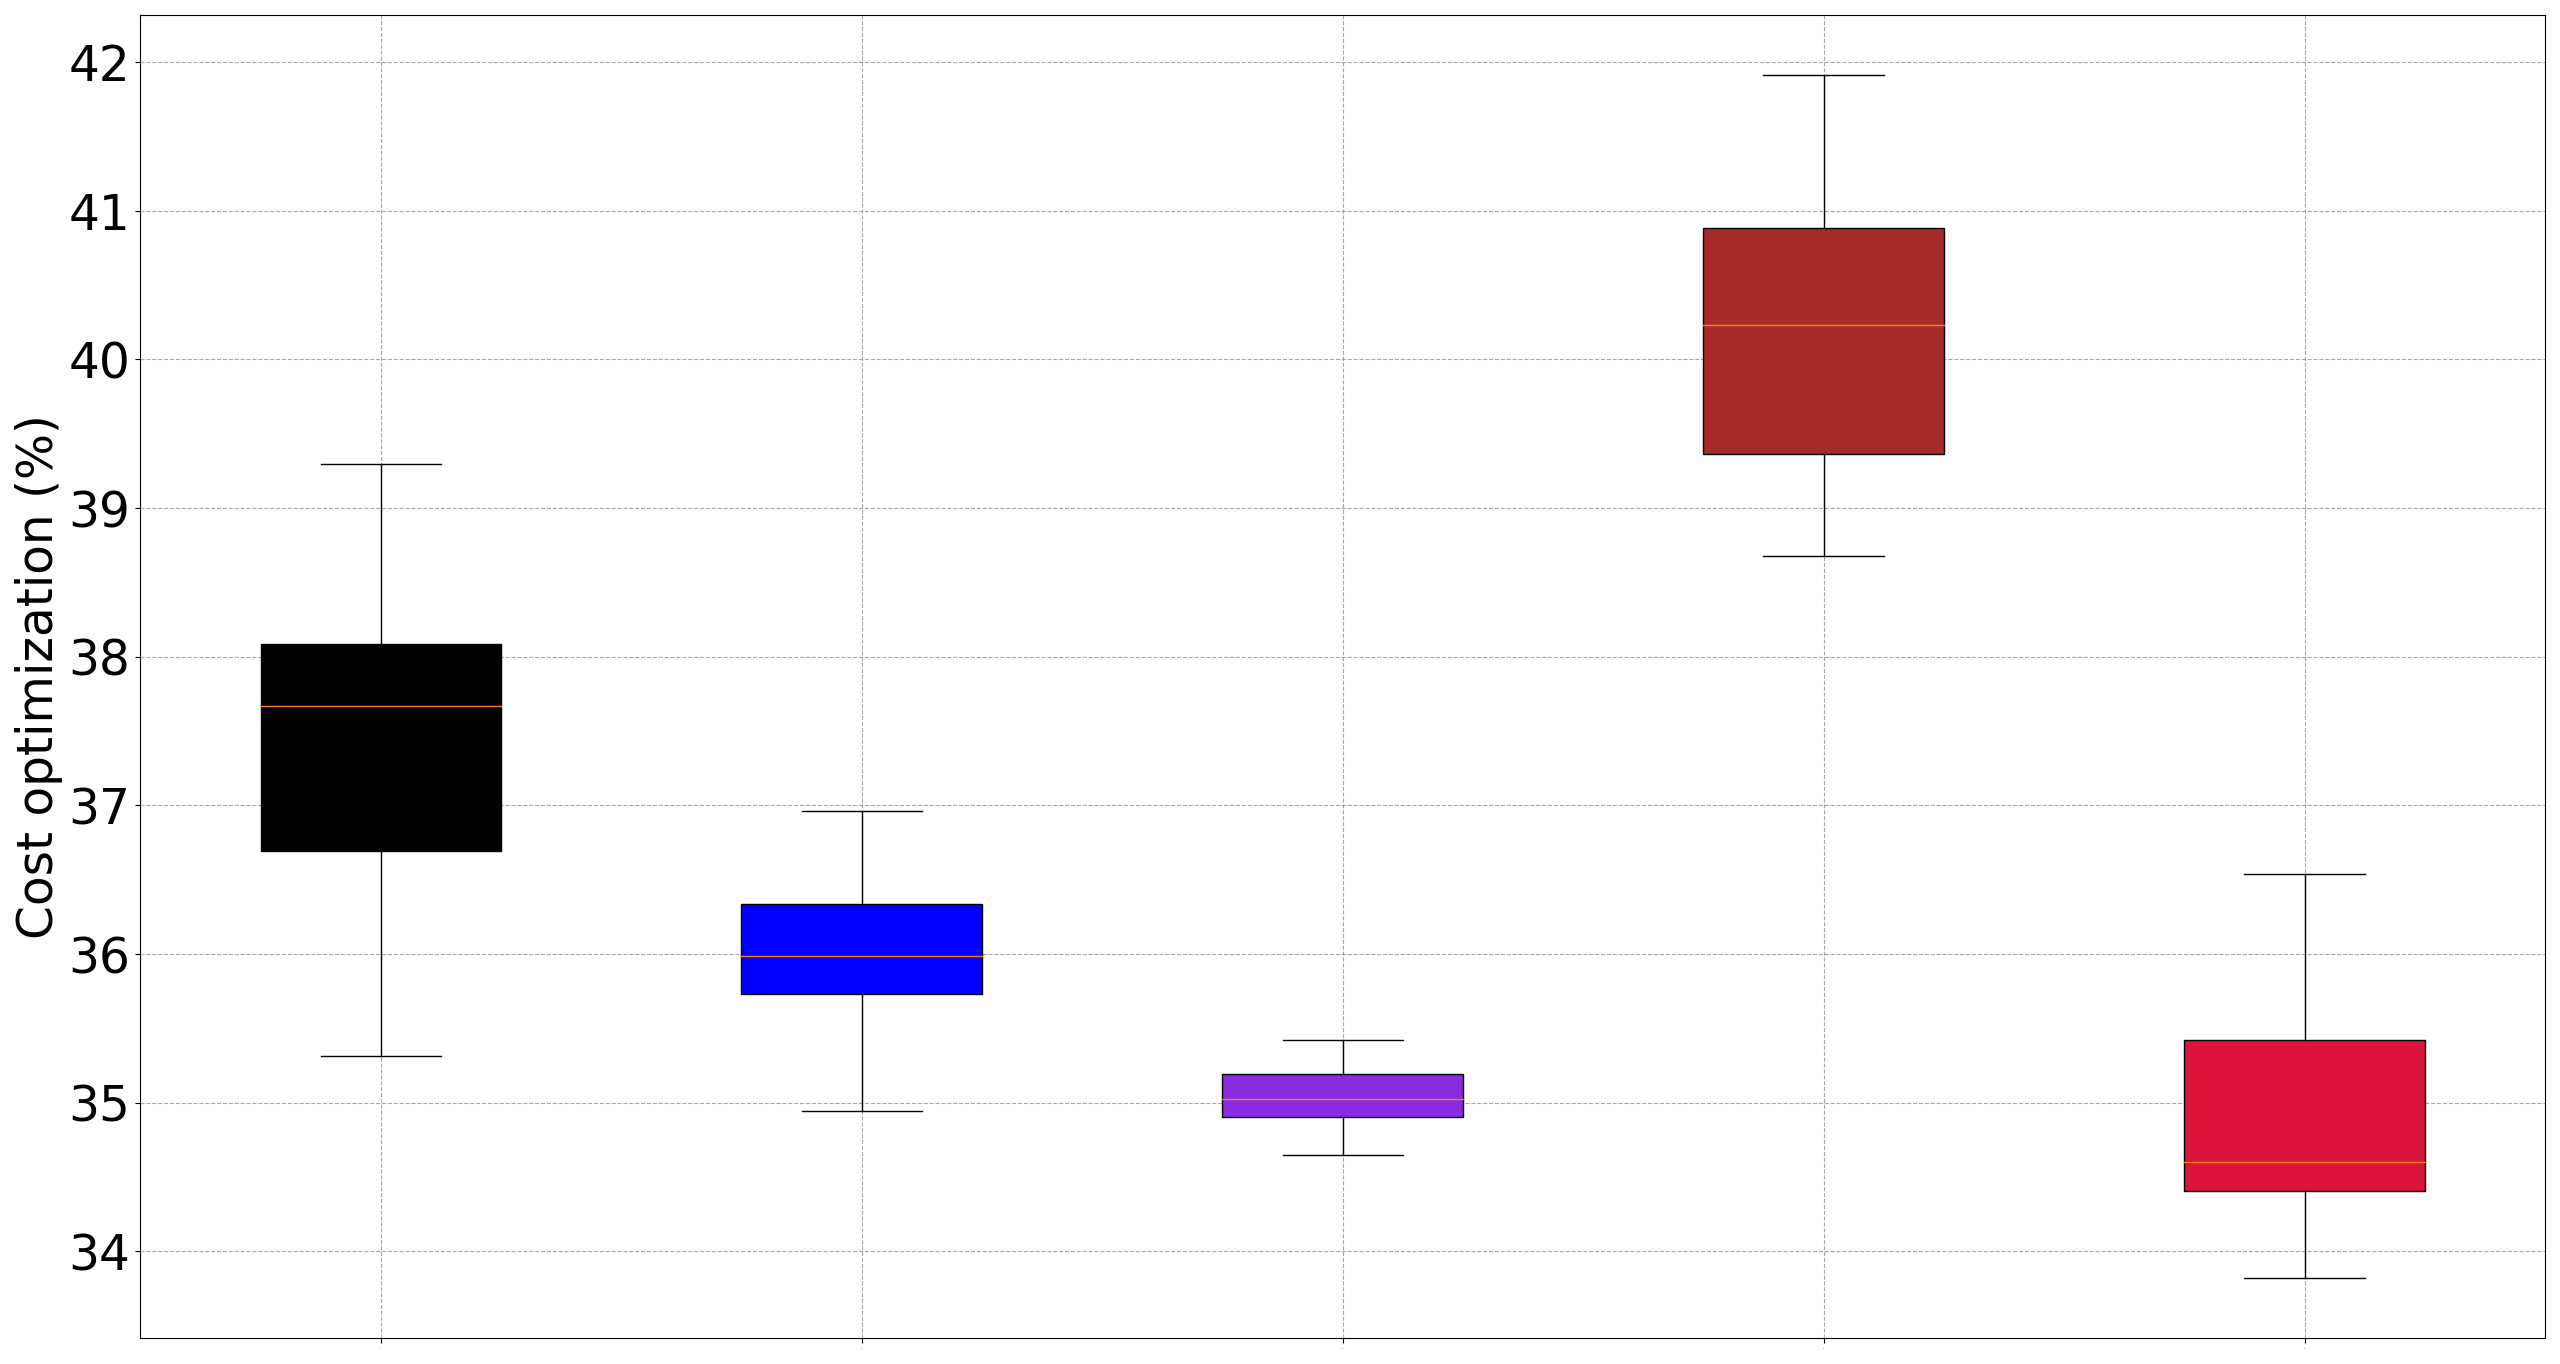
\includegraphics[width=0.9\linewidth]{figures/appendix/bplot_gaussian_radius_0_1.png}
    \caption{Cost optimization results using a Gaussian sampling with a standard deviation $\delta = 0.1$, averaged over 10 plans in a free space environment. 
    The standard deviation is represented as an envelope around the mean curves.
    The red curve corresponds to $K = 1$, the purple curve to $K = 2$, the blue one to $K = 3$, the black to $K = 5$, and the brown curve to $K = 10$.}%
    \label{fig:gaussian_radius_0_1}%
\end{figure}

\begin{figure} [htp]
    \centering
    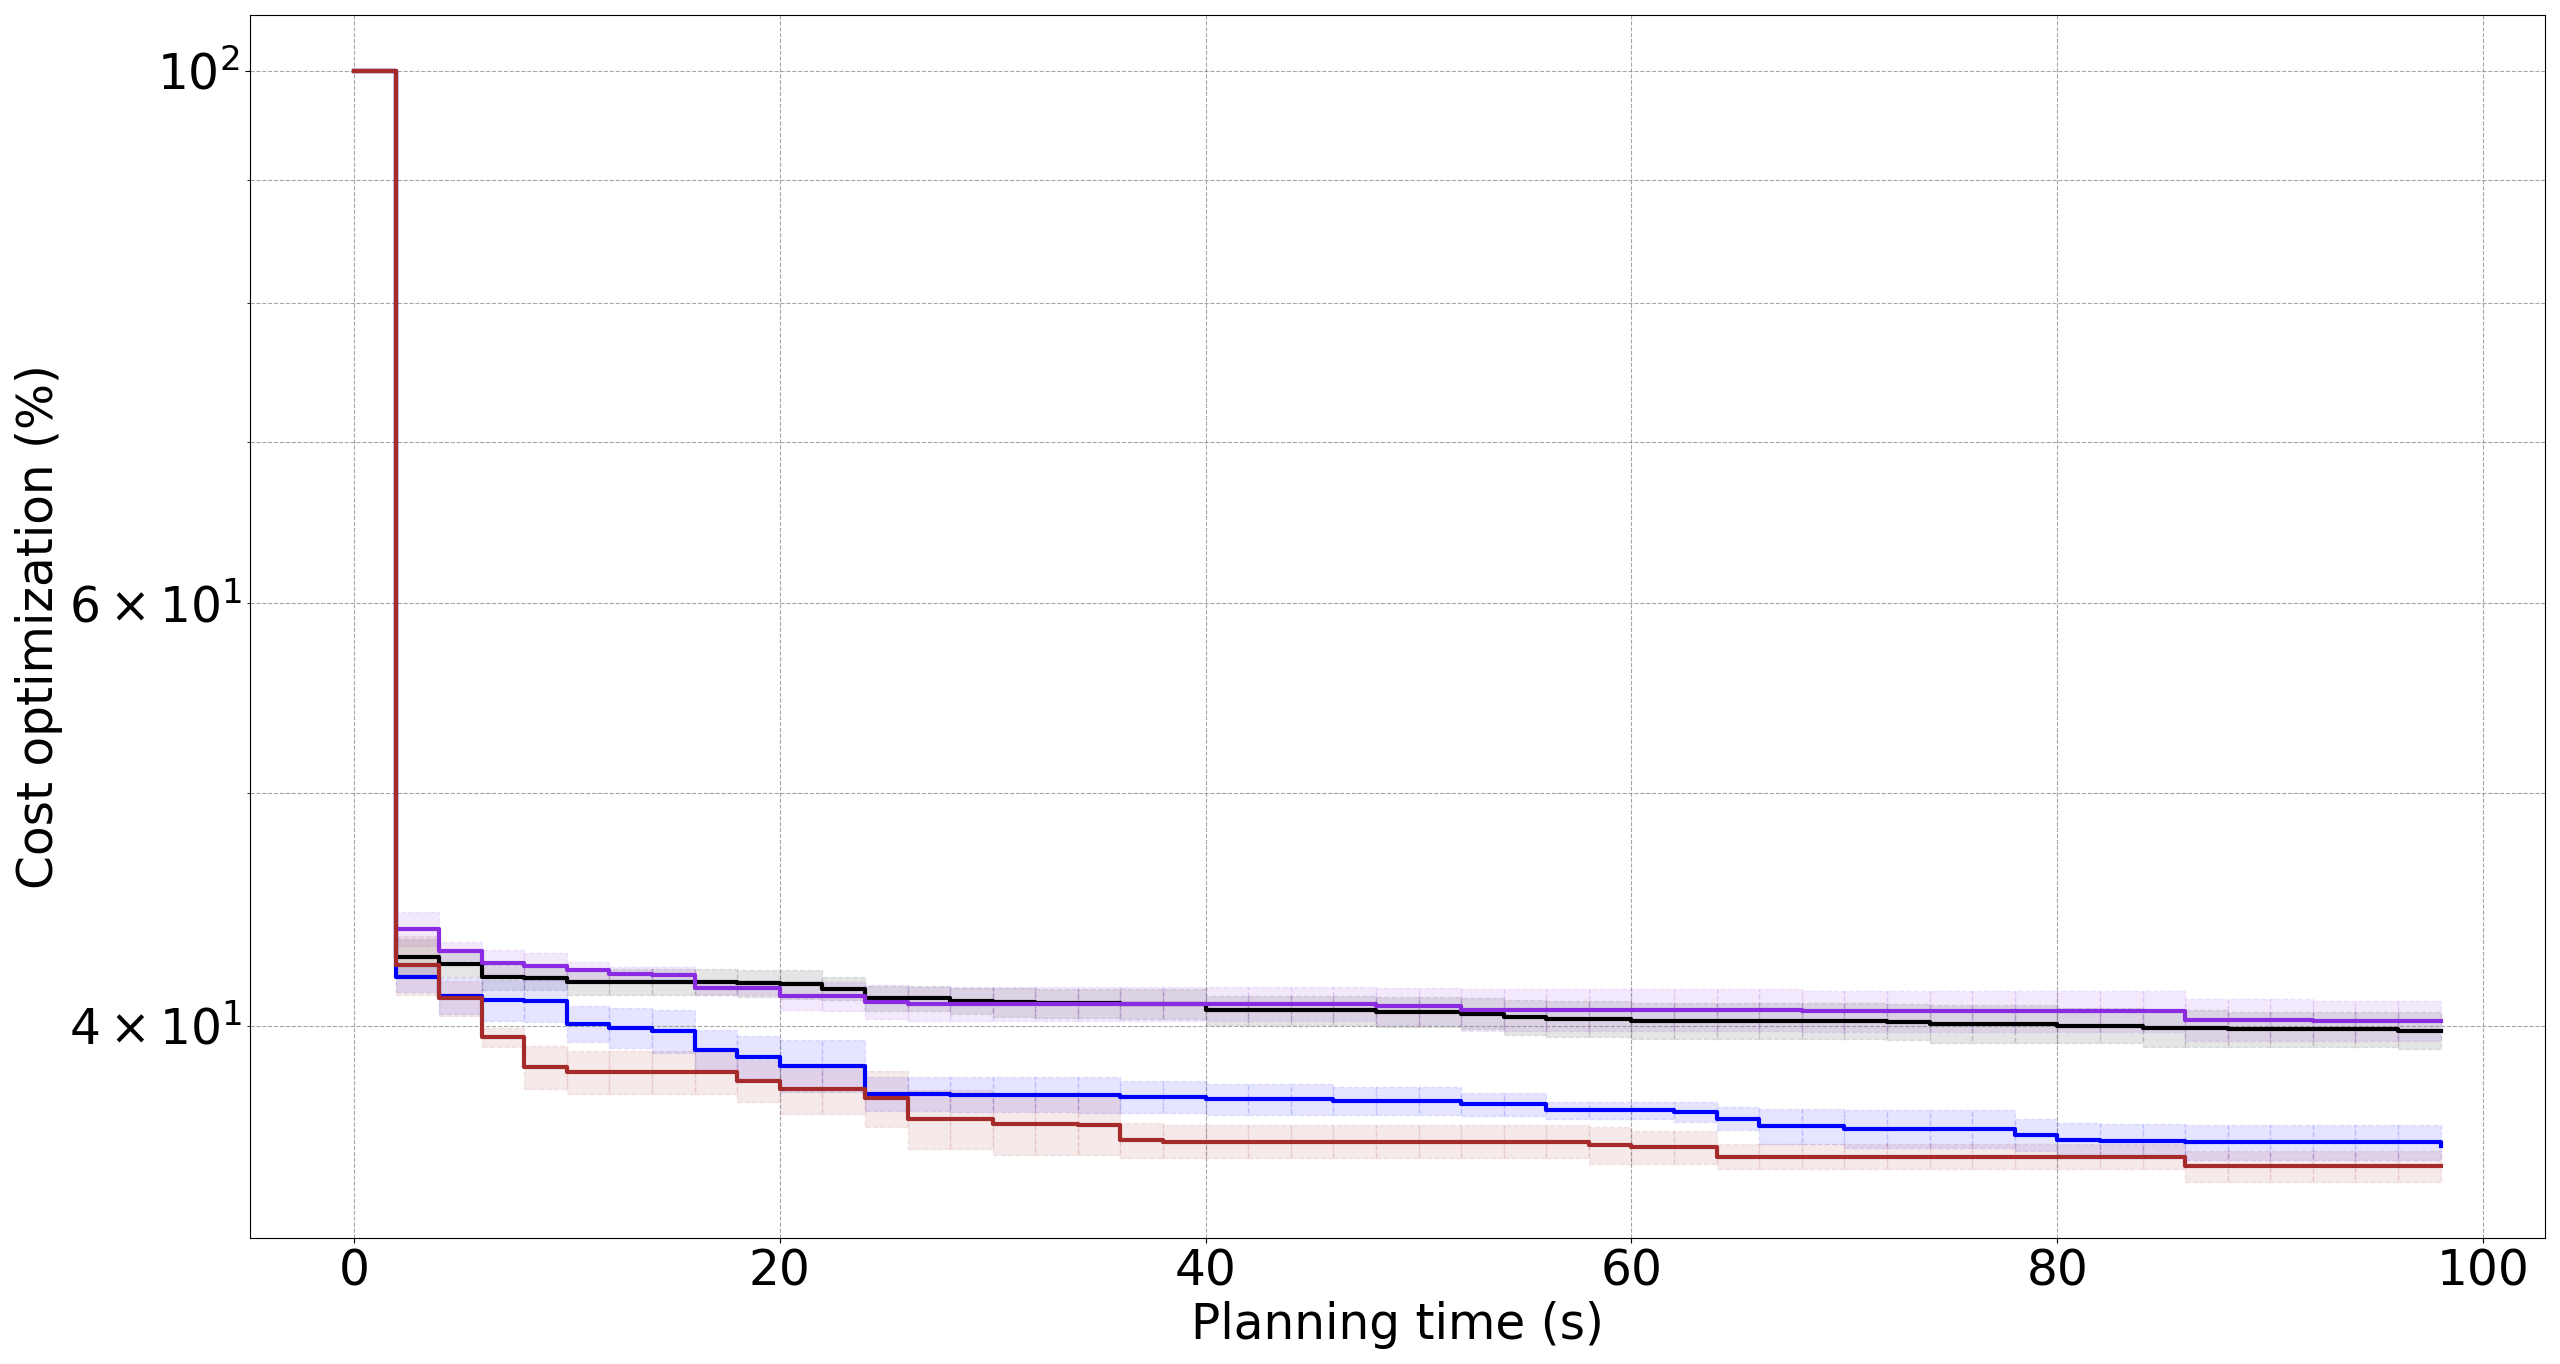
\includegraphics[width=0.9\linewidth]{figures/appendix/comp.png} \\
    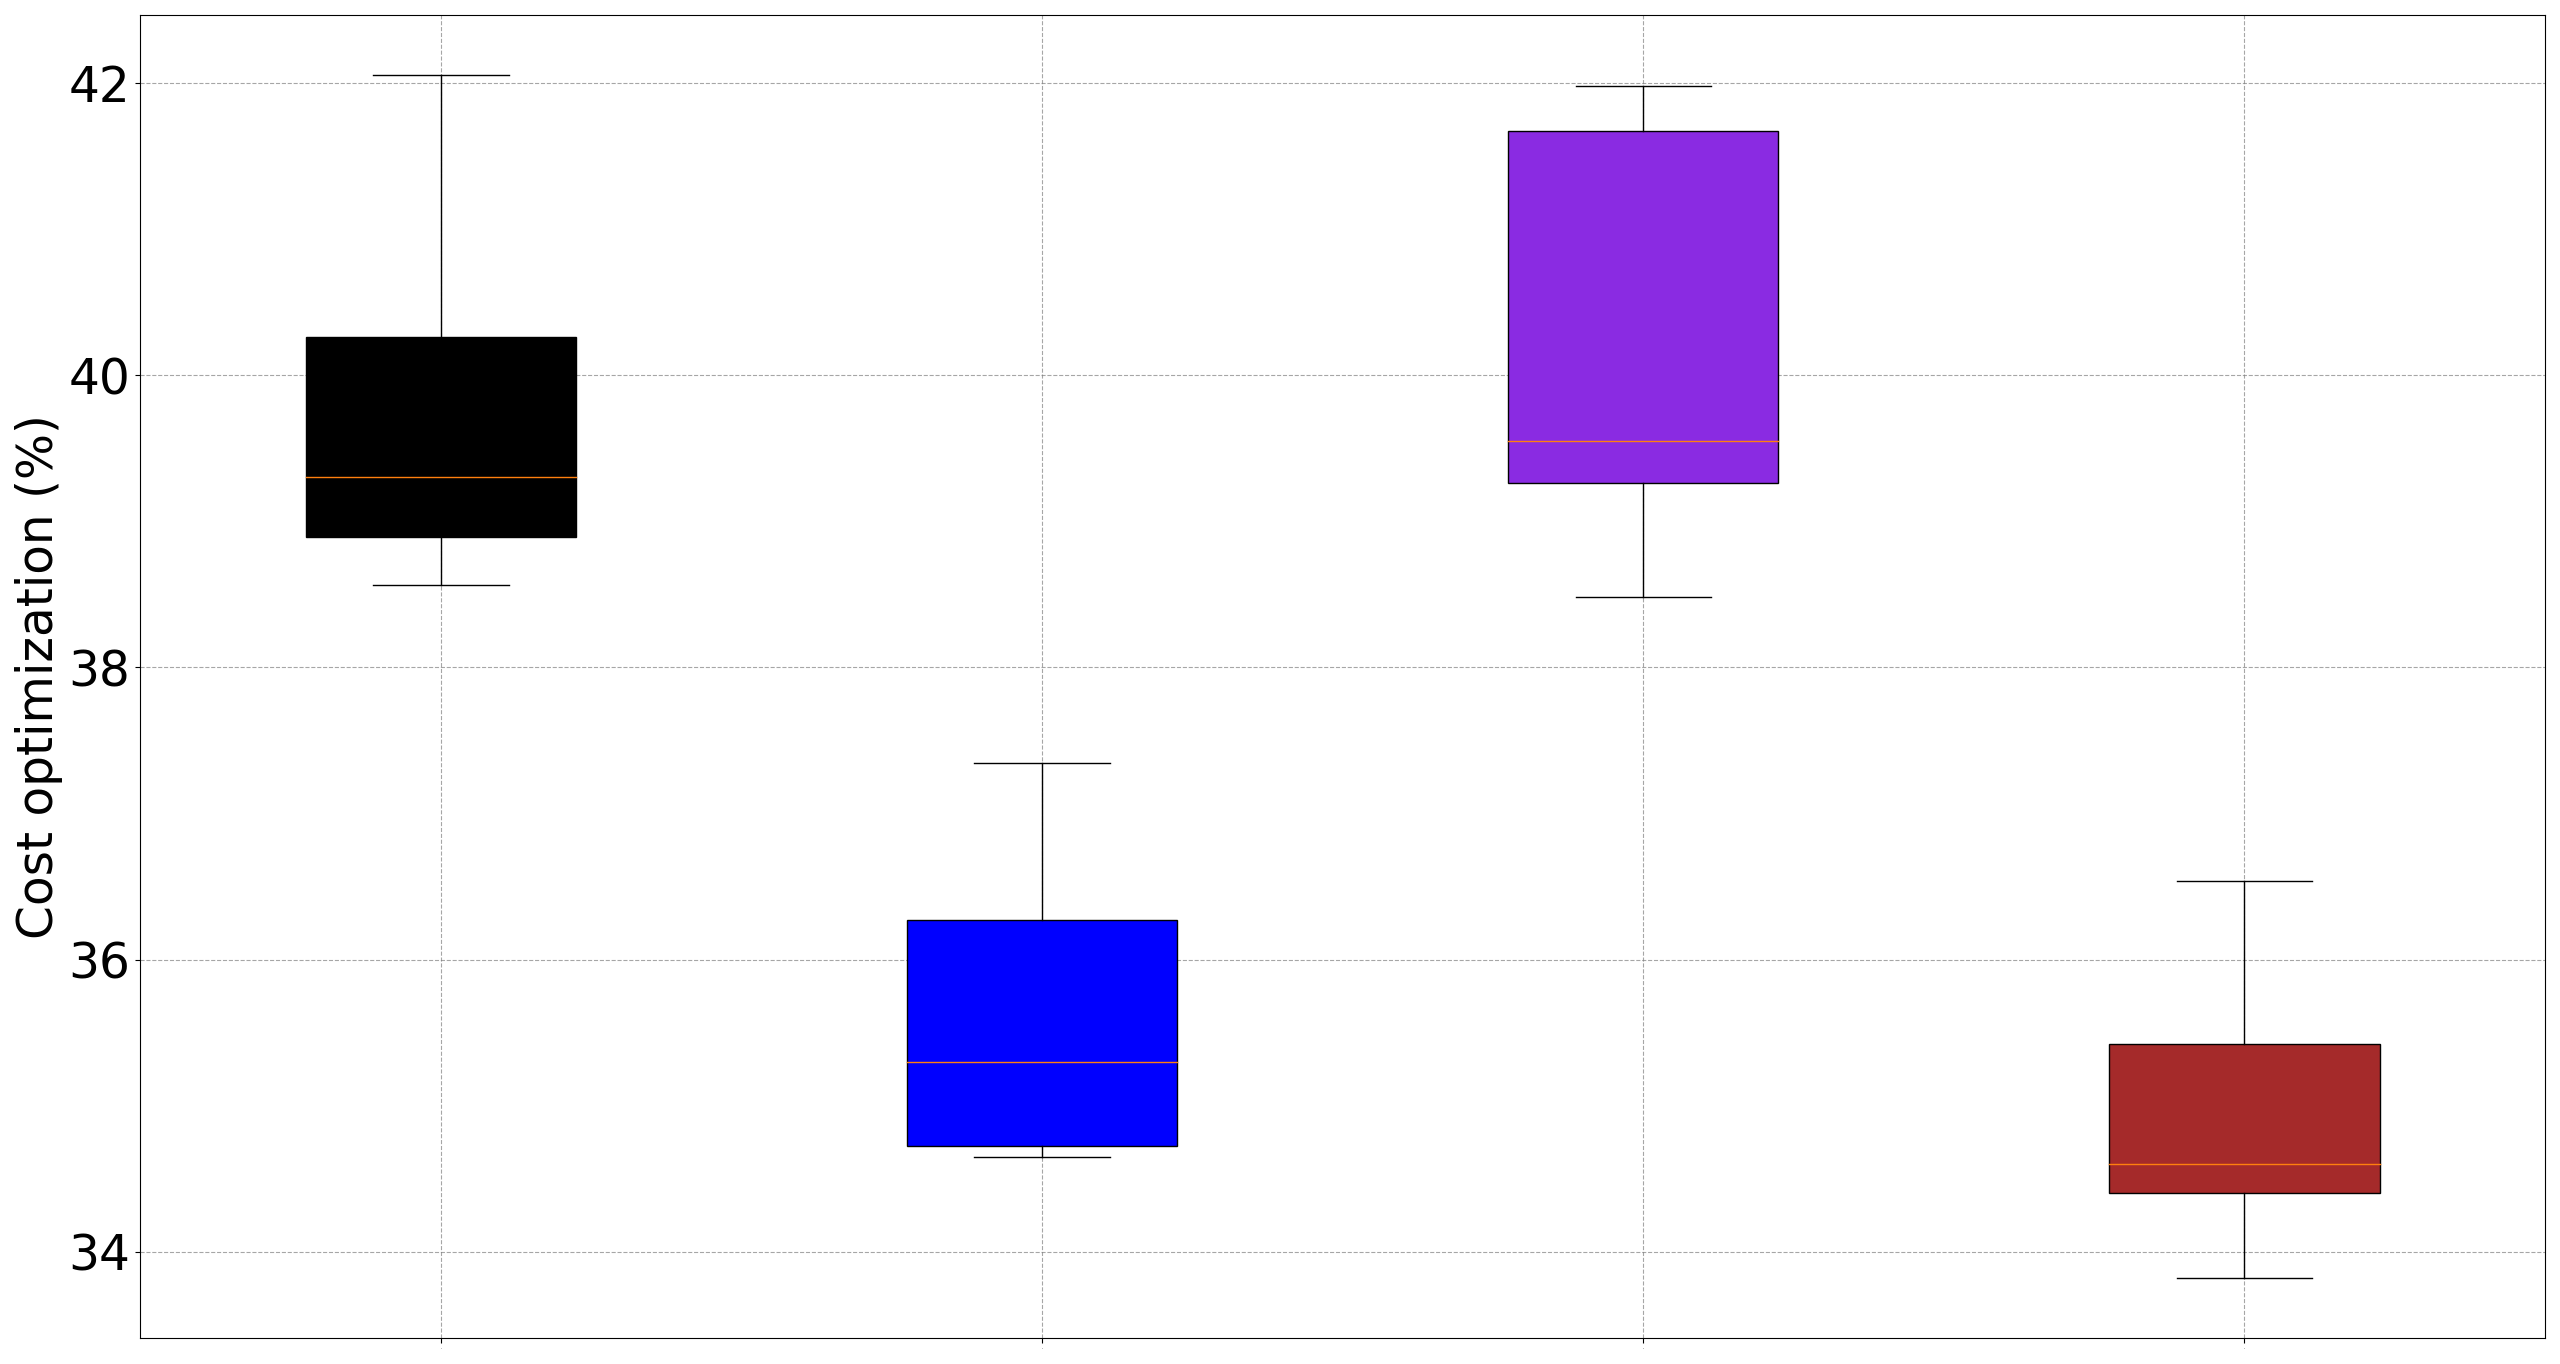
\includegraphics[width=0.9\linewidth]{figures/appendix/bplot_comp.png}
    \caption{Comparison of the best cases found in their respective classes: The red curve corresponds to a Gaussian sampling with $K = 1$ and $\delta = 0.1$, the blue curve is also associated to a Gaussian sampling with $K = 1$ and $\delta = 0.01$.
    The cases using uniform sampling are represented by the black and purple curves, both achieved with $K = 1$, and $\delta = 0.01$ and $\delta = 0.1$ respectively.}%
    \label{fig:comp}%
\end{figure}